\chapter{Contexte réglementaire et modélisation en assurance vie}
\label{chap:contexte}
\newpage
\section{Les spécificités des produits d'assurance vie épargne}
\label{sec:spec_av}

\subsection{Principes fondamentaux du contrat d'assurance vie}

L'assurance vie est une convention par laquelle un assureur, en contrepartie du versement de primes, s'engage à verser un capital ou une rente à la survenance d'un événement incertain lié à la durée de la vie humaine. Cet événement, qui constitue l'aléa au cœur du contrat, peut être le décès de l'assuré avant une date donnée ou, à l'inverse, sa survie jusqu'à cette date. Ce mécanisme repose sur un \textbf{cycle de production inversé} : l'assureur perçoit les primes bien avant de devoir potentiellement régler les prestations, ce qui l'amène à investir ces sommes sur des horizons de temps longs pour honorer ses engagements futurs.

\bigskip

La nature de ces engagements répond à des objectifs variés. Les contrats \textbf{en cas de vie} prévoient le versement d'un capital ou d'une rente à une échéance prévue si l'assuré est en vie ; ils sont typiquement utilisés pour se constituer un complément de retraite ou une épargne de précaution. À l'opposé, les contrats \textbf{en cas de décès} garantissent le versement d'un capital ou d'une rente au(x) bénéficiaire(s) désigné(s) au décès de l'assuré, souvent pour protéger des proches ou anticiper des droits de succession. Il existe également des contrats \textbf{mixtes} qui combinent ces deux garanties.

\bigskip

Le fonctionnement de ces contrats repose sur la \textbf{capitalisation} : les primes versées sont investies pour financer la propre couverture future de l'assuré. De par leur nature, ces engagements s'étendent sur de très longues périodes, conférant au passif de l'assureur une duration élevée, souvent supérieure à huit ans.

\bigskip

Une caractéristique fondamentale de l'assurance vie française est sa liquidité. L'assuré dispose de la possibilité de récupérer son épargne à tout moment via un \textbf{rachat}, qui peut être partiel ou total. Cette faculté de rachat constitue une option dont la valeur et le risque doivent être finement gérés par l'assureur, car son exercice a un impact direct sur la duration et les besoins de liquidité du portefeuille. La \textbf{fiscalité} joue un rôle incitatif majeur, les plus-values étant imposées plus lourdement si le rachat intervient avant la huitième année du contrat, encourageant ainsi l'épargne de long terme.

\subsection{Les principaux supports d'investissement}

L'épargne des assurés peut être investie sur deux principaux types de supports aux profils de risque distincts, qui peuvent être combinés au sein de différents types de contrats.

\bigskip

Le \textbf{fonds en euros} est le support historique et sécuritaire. Le risque financier y est intégralement porté par l'assureur, qui garantit à tout moment le capital investi. En conséquence, la politique d'investissement est prudente, majoritairement orientée vers des actifs peu risqués comme les obligations d'État (OATs) et d'entreprises (\textit{corporate bonds}), avec une portion résiduelle allouée aux actions ou à l'immobilier. Ce support est défini par plusieurs garanties. Le \textbf{taux technique} est un taux minimal de revalorisation garanti sur toute la durée du contrat, fixé à la souscription et soumis à un plafond réglementaire. En complément, l'assureur peut offrir un \textbf{Taux Minimum Garanti (TMG)}, similaire mais applicable sur une période plus courte (typiquement un ou deux ans). Enfin, l'effet "cliquet" assure que les revalorisations annuelles, composées du TMG et de la \textbf{Participation aux Bénéfices (PB)}, sont définitivement acquises. Pour lisser les performances, une partie de cette PB peut être mise en réserve dans une \textit{Provision pour Participation aux Bénéfices} (PPB), qui doit être redistribuée aux assurés dans un délai maximal de huit ans.

\bigskip

Les \textbf{unités de compte (UC)} offrent une exposition directe aux marchés financiers. Contrairement au fonds en euros, le risque d'investissement est entièrement porté par l'assuré. L'assureur ne garantit pas la valeur du capital, mais un nombre de parts d'actifs (OPCVM, actions, SCPI, etc.). La valeur de l'épargne fluctue ainsi au gré des marchés, offrant un potentiel de rendement supérieur à long terme, mais exposant également à un risque de perte en capital.

\bigskip

Ces supports sont proposés via deux grandes familles de contrats. Les contrats \textbf{monosupports} permettent d'investir sur un seul type de fonds (soit en euros, soit en UC). Les contrats \textbf{multisupports}, quant à eux, combinent au moins un fonds en euros et plusieurs supports en unités de compte, permettant à l'épargnant de répartir son investissement selon son profil de risque.
\textbf{Dans le cadre de cette étude, le portefeuille analysé se compose de contrats multisupports avec une répartition représentative du marché français, soit approximativement 60~\% en fonds euros et 40~\% en unités de compte.}

\subsection{Contexte économique et enjeux actuels}

La gestion de ces produits d'épargne est devenue particulièrement complexe dans l'environnement économique récent. Après une longue période de taux d'intérêt historiquement bas, le secteur de l'assurance a dû s'adapter à un nouveau paradigme marqué par une volatilité accrue et des taux durablement plus élevés.

\bigskip

Cette transition a mis les assureurs en difficulté. Leurs portefeuilles obligataires, constitués en grande partie d'anciennes obligations à faible rendement, présentent une forte inertie. Face à ce stock historique, il leur est difficile de générer des rendements suffisants pour offrir des taux de revalorisation attractifs sur les fonds en euros, capables de concurrencer les nouveaux produits de marché. Cet enjeu de compétitivité, couplé aux exigences de rentabilité et de solvabilité, place la gestion actif-passif au cœur des problématiques actuelles, justifiant pleinement l'introduction du cadre réglementaire qui suit.

\subsection{Les principaux supports d'investissement}

L'épargne des assurés peut être investie sur deux principaux types de supports aux profils de risque distincts.

\bigskip

Le \textbf{fonds en euros} est le support historique et sécuritaire. Le risque financier y est intégralement porté par l'assureur, qui garantit à tout moment le capital investi. En conséquence, la politique d'investissement est prudente, majoritairement orientée vers des actifs peu risqués comme les obligations. Ce support est défini par deux garanties majeures : le \textit{Taux Minimum Garanti} (TMG), fixé contractuellement, et l'effet "cliquet", qui assure que les revalorisations annuelles sont définitivement acquises. Au-delà du TMG, l'assureur a l'obligation de redistribuer une part de ses bénéfices techniques et financiers via la \textit{Participation aux Bénéfices} (PB). Pour lisser les performances, une partie de cette PB peut être mise en réserve dans une \textit{Provision pour Participation aux Bénéfices} (PPB), qui doit être redistribuée aux assurés dans un délai maximal de huit ans.

\bigskip

Les \textbf{unités de compte (UC)} offrent une exposition directe aux marchés financiers. Contrairement au fonds en euros, le risque d'investissement est entièrement porté par l'assuré. L'assureur ne garantit pas la valeur du capital, mais un nombre de parts d'actifs (OPCVM, actions, SCPI, etc.). La valeur de l'épargne fluctue ainsi au gré des marchés, offrant un potentiel de rendement supérieur à long terme, mais exposant également à un risque de perte en capital.

\section{Le cadre prudentiel Solvabilité II}
\label{sec:s2}

\subsection{Objectifs et structure de la norme}

Entrée en vigueur en 2016, la directive Solvabilité II a pour objectif d'harmoniser le régime de solvabilité des assureurs au sein de l'Union Européenne, afin d'optimiser la protection des assurés. Elle instaure une approche économique et prospective, fondée sur une évaluation fine et individualisée des risques. Cette approche se décline en trois piliers interdépendants.

\subsection{Le Pilier 1 : Exigences quantitatives}

Le Pilier 1 définit les règles de calcul des provisions techniques et du capital de solvabilité. Il impose une valorisation des actifs et des passifs en vision \textit{market-consistent}, c'est-à-dire cohérente avec leur valeur de marché, ce qui justifie l'utilisation d'un univers de projection risque neutre. Les principaux indicateurs réglementaires sont les suivants.

\bigskip

Le \textbf{Best Estimate (BE)}, ou \textit{Best Estimate Liability} (BEL), représente la meilleure estimation de la valeur actuelle des flux de trésorerie futurs liés aux engagements d'assurance. Son calcul est réalisé dans l'hypothèse d'un portefeuille en extinction (\textit{run-off}), c'est-à-dire sans l'ajout de nouveaux contrats. Il est obtenu par la moyenne des flux actualisés sur un grand nombre de simulations économiques stochastiques en univers risque neutre~:
\begin{equation}
    BEL = \mathbb{E}^{\mathbb{Q}} \left[ \sum_{j=1}^{T} CF(j) \cdot e^{-\int_0^j r(s)ds} \right] \approx \frac{1}{N}\sum_{i=1}^{N}\sum_{j=1}^{T}\frac{CF_{i}(j)}{(1+r_{i,j})^{j}}
\end{equation}
Où $N$ est le nombre de simulations, $T$ l'horizon de projection, $CF_{i}(j)$ le flux de trésorerie net de l'année $j$ pour la simulation $i$, et $r_{i,j}$ le taux d'actualisation sans risque pertinent.

\bigskip

La \textbf{Marge de Risque (Risk Margin - RM)} s'ajoute au Best Estimate pour couvrir le coût de détention du capital réglementaire associé aux risques non-financiers (ou non-couvrables). Elle est calculée selon une approche "Coût du Capital" (\textit{Cost of Capital} - CoC), correspondant à la valeur actuelle des coûts futurs liés à l'immobilisation du capital réglementaire requis pour ces risques~:
\begin{equation}
    RM = \text{CoC}_{\text{rate}} \times \sum_{j=0}^{T} \frac{\text{SCR}_{\text{non-fi}}(j)}{(1+r_{j+1})^{j+1}}
\end{equation}
Où $\text{CoC}_{\text{rate}}$ est le coût du capital (fixé à 6\%), $\text{SCR}_{\text{non-fi}}(j)$ est la part du SCR couvrant les risques non-financiers à l'année $j$ en \textit{run-off}, et $r_{j+1}$ est le taux sans risque à l'échéance $j+1$.

\bigskip

Le \textbf{Solvency Capital Requirement (SCR)} est le montant de fonds propres (ou \textit{Net Asset Value} - NAV) nécessaire pour faire face à une perte inattendue et sévère, calibré pour correspondre à une Value-at-Risk (VaR) à 99,5\% à un horizon d'un an. En formule standard, son calcul suit une approche modulaire. Pour un risque élémentaire $x$, le SCR est défini comme la perte de fonds propres résultant de l'application d'un choc calibré~:
\begin{equation}
    SCR_{x} = NAV_{\text{central}} - NAV_{\text{choc}}
\end{equation}
En partant de l'équation de bilan simplifiée $Actifs_{VM} = BE + RM + NAV$, et en supposant la Marge de Risque constante lors du choc, la perte de NAV est égale à la variation du surplus des actifs sur le BE~:
\begin{equation*}
    SCR_{x} = (Actifs_{VM}^{\text{central}} - BE^{\text{central}}) - (Actifs_{VM}^{\text{choc}} - BE^{\text{choc}})
\end{equation*}
Pour les risques de passif purs (mortalité, longévité, rachat), le choc n'affecte par définition que les flux de passif. La valeur des actifs reste donc inchangée ($Actifs_{VM}^{\text{central}} = Actifs_{VM}^{\text{choc}}$), et la formule se simplifie en une variation de Best Estimate~:
\begin{equation*}
    SCR_{\text{passif}} = BE^{\text{choc}} - BE^{\text{central}} = \Delta BE
\end{equation*}
En revanche, pour les risques de marché, le choc affecte à la fois les actifs et le passif (via les taux d'actualisation), rendant indispensable le calcul de la variation de la NAV dans sa totalité.

\bigskip

Les SCR des risques élémentaires sont ensuite agrégés en modules (marché, souscription, etc.) à l'aide de matrices de corrélation, puis ces modules sont à leur tour agrégés pour former le SCR final, après ajustement pour la capacité d'absorption des impôts et l'ajout du risque opérationnel.
\begin{equation}
    SCR_{\text{marché}} = \sqrt{\sum_{i,j} \rho_{ij}^{\text{marché}} \cdot SCR_i \cdot SCR_j}
\end{equation}

\bigskip

\begin{equation}
    BSCR = \sqrt{\sum_{i,j} \rho_{ij}^{\text{global}} \cdot SCR_{\text{module}, i} \cdot SCR_{\text{module}, j}}
\end{equation}

\bigskip

\begin{equation}
    SCR = BSCR - Adj + SCR_{op}
\end{equation}

\bigskip

\begin{figure}[H]
    \centering
    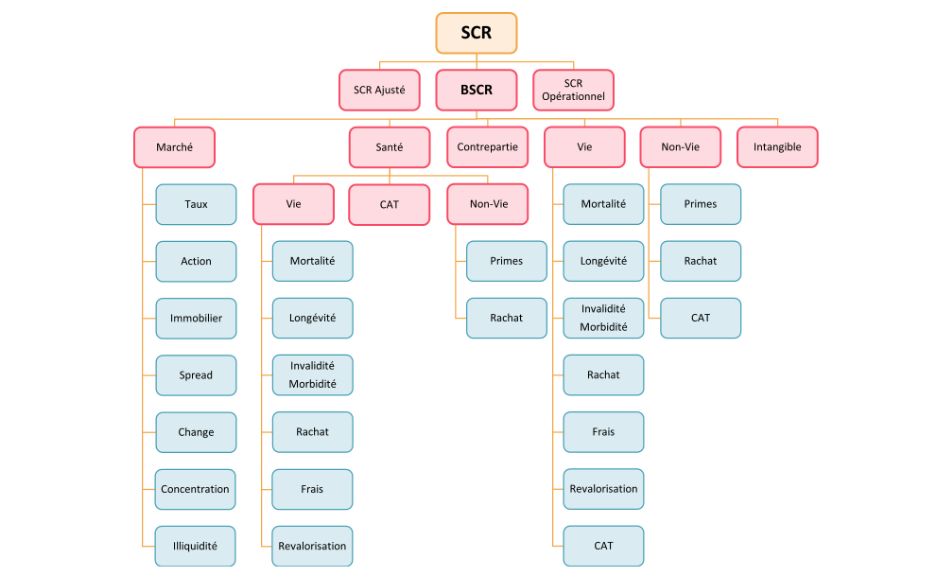
\includegraphics[width=0.95\textwidth]{images/pieuvre_scr.png}
    \caption{Schéma des modules et sous-modules du SCR}
    \label{fig:pieuvre_scr}
\end{figure}

\subsection{Le Pilier 2 : Exigences qualitatives et gouvernance}

Au-delà des exigences quantitatives, le Pilier 2 se concentre sur la supervision des risques et la gouvernance interne. Il impose aux assureurs de mettre en place un \textbf{système de gouvernance} efficace, incluant une structure organisationnelle transparente, des politiques écrites claires et un système de contrôle interne robuste. Ce système doit s'articuler autour de quatre \textbf{fonctions clés} indépendantes : la fonction actuarielle, la gestion des risques, l'audit interne et la conformité.

\bigskip

L'élément central du Pilier 2 est l'\textbf{ORSA} (\textit{Own Risk and Solvency Assessment}). Il s'agit d'un processus interne et prospectif par lequel l'assureur évalue, sur un horizon de moyen terme (généralement 3 à 5 ans), l'adéquation entre son profil de risque spécifique, ses limites de tolérance au risque et ses besoins globaux en solvabilité, au regard de sa stratégie d'entreprise. L'ORSA n'est pas un simple exercice de calcul, mais un véritable outil de pilotage stratégique qui contraint l'assureur à analyser des scénarios et des risques qui lui sont propres, allant au-delà des exigences standard du Pilier 1.

\subsection{Le Pilier 3 : Exigences de reporting et transparence}

Le Pilier 3 vise à assurer la transparence et l'harmonisation de l'information financière à destination du public et des autorités de contrôle, complétant ainsi les deux premiers piliers par une obligation de communication rigoureuse.

\bigskip

D'une part, il instaure une \textbf{communication publique} à travers la publication annuelle d'un rapport sur la solvabilité et la situation financière, le \textit{Solvency and Financial Condition Report} (SFCR). Ce document public détaille la performance de l'entreprise, son système de gouvernance, son profil de risque, ainsi que les méthodes de valorisation et de gestion du capital utilisées.

\bigskip

D'autre part, il définit un \textbf{reporting au superviseur} beaucoup plus détaillé. Les assureurs doivent remettre périodiquement (trimestriellement et annuellement) des informations quantitatives granulaires via des formats standardisés, les \textit{Quantitative Reporting Templates} (QRT). Ils soumettent également un rapport narratif confidentiel, le \textit{Regular Supervisory Report} (RSR), ainsi que le rapport issu de leur processus ORSA, permettant à l'autorité de contrôle d'exercer sa mission de supervision.

\section{La gestion Actif-Passif (ALM) : définitions et enjeux}
\label{sec:alm}

La gestion Actif-Passif, ou \textit{Asset-Liability Management} (ALM), est la discipline qui vise à piloter de manière coordonnée l'actif et le passif du bilan d'un assureur. L'enjeu fondamental de l'ALM découle directement du \textbf{cycle de production inversé} : les primes sont collectées et investies bien avant que les prestations ne soient versées. Ce décalage temporel crée une \textbf{inadéquation} (\textit{mismatch}) structurelle entre les caractéristiques des actifs (soumis à la volatilité des marchés) et celles des passifs (de longue durée et parfois assortis de garanties).

\bigskip

L'objectif de l'ALM est donc de gérer activement les risques découlant de cette inadéquation, notamment le \textbf{risque de taux d'intérêt}, le \textbf{risque de liquidité} (lié aux rachats) et les \textbf{risques de marché} (actions, crédit), afin de s'assurer que les flux générés par les actifs seront suffisants pour honorer les engagements, tout en optimisant la rentabilité et en respectant les contraintes réglementaires.

\bigskip

Pour ce faire, les assureurs s'appuient sur des \textbf{modèles ALM} sophistiqués. Ces modèles simulent l'évolution conjointe de l'actif et du passif sur des horizons de temps longs (40 ans ou plus), sous une multitude de scénarios économiques. Ils intègrent les caractéristiques des portefeuilles, les lois de comportement des assurés (rachats, mortalité) et les règles de gestion de l'assureur (politique de PB, stratégie de couverture). Ces projections permettent d'évaluer l'impact de différentes stratégies et constituent un outil indispensable à la prise de décision.

\section{Les Générateurs de Scénarios Économiques (GSE)}
\label{sec:gse}

Le moteur de tout modèle ALM est le \textbf{Générateur de Scénarios Économiques (GSE)}, un outil mathématique qui simule de multiples trajectoires futures cohérentes pour un ensemble de variables économiques (taux d'intérêt, cours des actions, inflation, etc.). La robustesse des projections ALM dépend directement de la qualité du calibrage du GSE, qui s'appuie sur des données de marché à une date donnée. Deux cadres de projection distincts coexistent.

\bigskip

L'\textbf{univers Risque Neutre ($\mathbb{Q}$)} est un cadre de valorisation théorique, indispensable pour les calculs réglementaires \textit{market-consistent} sous Solvabilité II. Sous l'hypothèse d'absence d'opportunité d'arbitrage, il existe une probabilité unique, dite "risque neutre", sous laquelle le rendement espéré de tout actif est égal au taux sans risque. Les prix actualisés des actifs y sont des martingales.

\bigskip

L'\textbf{univers Monde Réel ($\mathbb{P}$)} vise à représenter les anticipations réelles de l'évolution de l'économie. Les rendements espérés des actifs y intègrent des primes de risque (actions, crédit) pour rémunérer les investisseurs. Ce cadre est utilisé pour le pilotage stratégique, le \textit{business plan} et les analyses prospectives de l'exercice ORSA.


\section{La représentation du passif : le concept de \textit{Model Point}}
\label{sec:mp}

\subsection{La nécessité de l'agrégation}

Les portefeuilles d'assurance vie comptent souvent des centaines de milliers, voire des millions de polices. Une modélisation "police à police" est techniquement possible mais informatiquement irréalisable pour des calculs stochastiques complexes comme ceux requis par les modèles ALM. La charge de calcul deviendrait prohibitive. La simplification du portefeuille de passif n'est donc pas un choix, mais une contrainte opérationnelle fondamentale.

\bigskip

La réponse standard à cette contrainte est la création de \textbf{\textit{Model Points}} (MP). Un MP est un contrat synthétique représentant un agrégat de polices partageant des caractéristiques homogènes. L'objectif est de réduire drastiquement le volume de données à traiter tout en préservant les propriétés actuarielles et financières essentielles du portefeuille complet. La qualité de la représentation dépend directement de la pertinence des critères de regroupement (caractéristiques du produit, de l'assuré, du contrat), souvent optimisés par des techniques de classification statistique (\textit{clustering}).

\subsection{Du Model Point à la problématique du mémoire}

L'utilisation des \textit{Model Points} constitue la méthode standard pour agréger le passif et rendre les modèles ALM opérationnels. Cependant, la manière dont ces groupes de contrats sont formés à partir des polices individuelles a un impact direct et significatif sur la valorisation des indicateurs réglementaires et leur sensibilité aux chocs.

\bigskip

La problématique centrale de ce mémoire est donc d'optimiser cette étape fondamentale de l'agrégation. En partant du portefeuille granulaire "police à police", nous cherchons à définir, comparer et tester différentes méthodes de regroupement pour créer des \textit{Model Points}. L'objectif est de construire une méthodologie de simplification optimale, c'est-à-dire celle qui minimise l'erreur d'agrégation tout en garantissant la plus grande stabilité des indicateurs Solvabilité II (SCR, Marge de Risque, NAV) lors du calcul des différentes sensibilités. Cette section introductive pose donc les fondations de notre analyse : la simplification étant une nécessité, comment s'assurer que la méthode de regroupement choisie est la plus fidèle et la plus robuste possible ?
